\documentclass[UTF8]{article}
\usepackage{cite}
\usepackage[unicode,pdftex]{hyperref}
\usepackage{enumerate}
% \usepackage{geometry}
\usepackage{setspace}
\usepackage{pslatex} 
\usepackage{fancyhdr}
\usepackage{float}
\usepackage{amsmath}
\usepackage{titling}
\usepackage{indentfirst}
\usepackage{graphicx}
\usepackage{wrapfig}
\usepackage{amsmath}
\usepackage{xstring}
\usepackage{tikz}
\usetikzlibrary{fit, calc}
\pagestyle{empty} 



% \geometry{left=2.5cm, right=2.5cm, top=1.4cm, bottom=2.4cm}
\usepackage[a4paper,top=1.4cm,bottom=2cm,left=3cm,right=3cm,marginparwidth=1in, margin=1in]{geometry}
% \usepackage[margin=1in]{geometry}
\title{ Deep Distribution Learning for Vessel Extraction}
\author{Chenqiu Zhao(zhao.chenqiu@ualberta.ca)}
\date{}


\newcommand{\reffig}[1]{Fig. \ref{#1}}
\newcommand{\refsec}[1]{Section \ref{#1}}
% \newcommand{\refeq}[1]{Eq. \ref{#1}}
\newcommand{\reftab}[1]{Table \ref{#1}}


\fancyhead{}
\lhead{\scriptsize Chenqiu Zhao}
\rhead{\scriptsize research Proposal}

\renewcommand{\headrulewidth}{0pt}
\renewcommand{\normalsize}{\fontsize{12pt}{\baselineskip}\selectfont}


\newcommand{\chronoperiode}[7]{
  \pgfmathsetmacro{\first}{(#2 - 2018)*12 + #3 - .9} % beginig of the peropd
  \pgfmathsetmacro{\last}{(#4 - 2018)*12 + #5 - 1.1} % end of the period
  \pgfmathsetmacro{\middle}{(\first+\last)/2} % position of the country name
  \fill[#7] (\first,#6-1) rectangle (\last,#6) (\middle,#6-.5) node[white, font=\sf]{#1};
}

\definecolor{level1}{RGB}{200,10,20}
\definecolor{brightube}{rgb}{0.82, 0.62, 0.91}
\definecolor{fuchsia}{rgb}{1.0, 0.0, 1.0}
\definecolor{heliotrope}{rgb}{0.87, 0.45, 1.0}

\geometry{left=3cm,right=2.5cm,top=0.5cm,bottom=2.5cm}

\begin{document}

\maketitle
%\vspace{-90pt}


\vspace{-30pt}


\section*{Abstract}
Is there any better way rather than histograms can be utilized to classify two distributions,
\textbf{can we make the deep learning network learn and classify distributions automatically and accurately,}
which should have a wide range of applications in computer vision, such as moving objects segmentation, border extraction or Vessel Extraction.
%
In our previous work \cite{2018_ICME_8486510},
we already found that the convolutional neural network can be forced to focus on statistical distribution
by randomly permutating the input of network.
%
Such property is utilized to segment moving objects in a video.
since the distribution generated by moving objects has a significant difference with the ones of background scenes.
%
Fortunately,
such phenomenons are also shown in Vessel Extraction.
%
Therefore,
in this proposal,
we want to extend this technique to vessel extraction.
In addition,
we also want to drag deeper into this field to figure out what exactly learned by the network.
%
why the network acquires the ability to classify the statistical distribution theoretically.
% does the network can recognize a particular distribution, or several different distributions.
%
We will focus on improving the performance as well as the generality of distribution learning.
In particular,
the theoretical procedure will be a key task in this proposal,
since it is very important for academia.
%
Also,
once we figure out the reason for the network's ability to classify distributions,
it is also helpful to devise a better network for distribution learning.

\vspace{-10pt}
\section*{Introduction}
\begin{wrapfigure}{l}{0.4\textwidth}
%  \vspace{-15pt}    % 对应高度1
  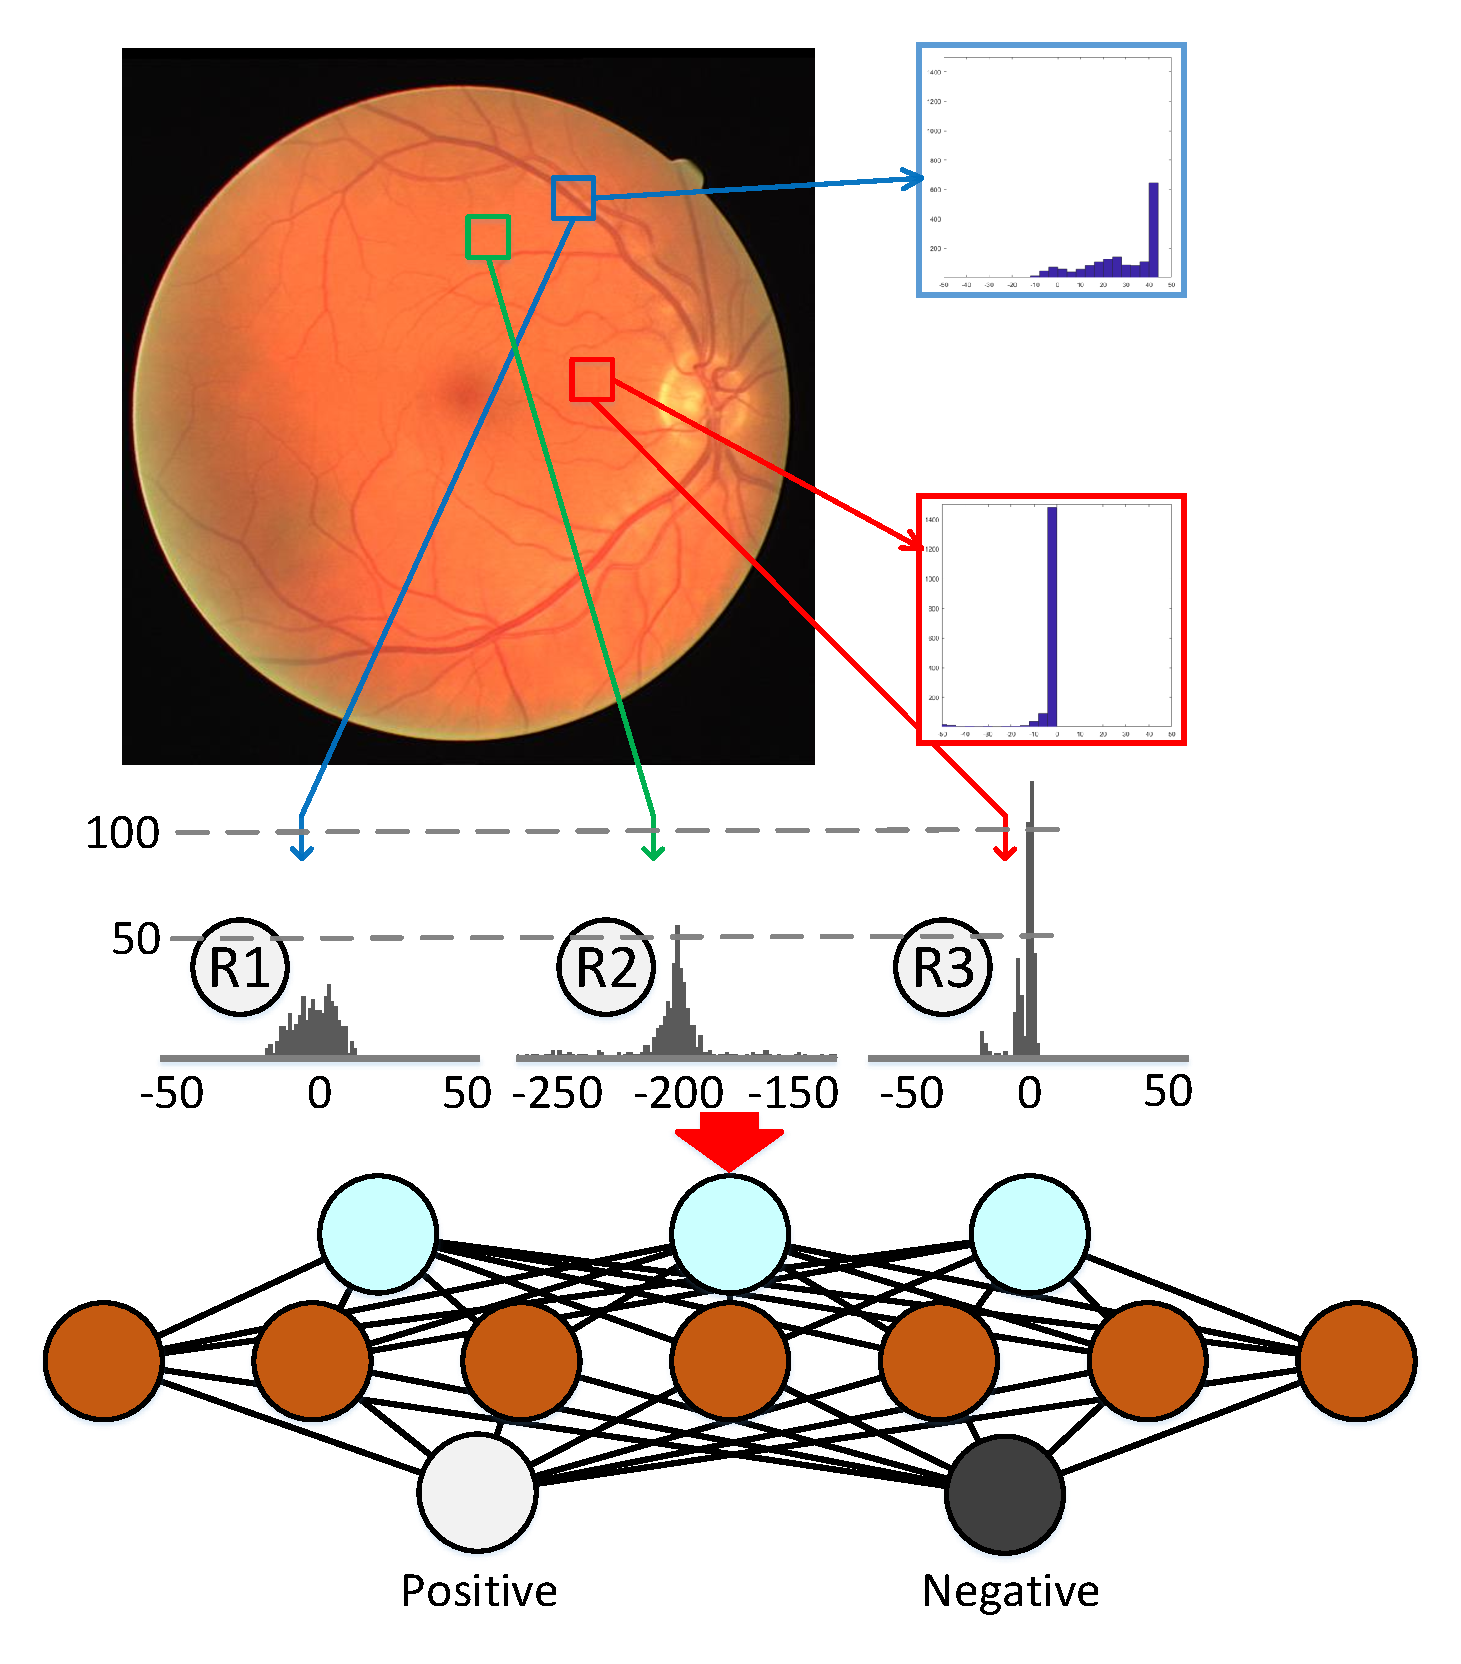
\includegraphics[width=0.4\textwidth]{figure/fig1.pdf}\\
    \label{fig1}
%  \vspace{-15pt}    % 对应高度2
  \caption{Deep distribution Learning.}
    \label{fig1}
%  \vspace{-15pt}    % 对应高度3
\end{wrapfigure}


% \begin{figure}[!h]
%     \centering
%     \includegraphics[width=0.5\textwidth]{../imgs/distribution.pdf}
%     \caption{Segmenting moving objects in freely moving camera.}
%     \label{fig_intro}
% \end{figure}

Traditionally,
the histogram is one of the most popular techniques for analyzing distributions.
%
People captured the histograms of distributions to describe, classify and understand the distributions from data.
%
However,
histograms of distributions are kinds of low-level features such as the features learned by the first layer of the convolutional neural network.
%
In our previous work,
we already proposed that by randomly permutating the input of the convolutional neural network,
the network can be forced to focus on statistical distribution.
%
This distribution learning method was applied to background subtraction and achieves promising results \cite{2018_ICME_8486510}.
%
Now, we are trying to extend the applications of our distribution learning method,
and apply the method to vessel extraction,
which is shown as \reffig{fig1},
since the distribution around pixels in the vessel has obvious difference compared with the pixels outside the vessel.
%
Moreover,
like the hierarchical features learned by deep learning networks,
which work better than all these artificial features,
\textbf{is there any hierarchical representation of distribution implied which is not be discovered yet?}
%
\textbf{Will this high-level distribution work better than the existing techniques, e.g. histogram, density estimation and so on, related to distribution?}
%
Solving this problem would be extremely interesting, which is the \textbf{main purpose of "\textcolor{red}{Deep} Distribution Learning".}



\small
\bibliographystyle{unsrt}
% \bibliographystyle{plain}
\bibliography{ref.bib}  




\end{document}
